% When editing in the supplied SPS template, keep its ieeeconf.cls next to this file.
% A checkout without the course class builds in standard IEEE conference format.
\IfFileExists{./ieeeconf.cls}{\documentclass[9pt]{ieeeconf}}{\documentclass[conference]{IEEEtran}\usepackage[T1]{fontenc}}
\usepackage{amsmath,graphicx,booktabs,url}
\title{PRoCoP: Placement-Based Routing Congestion Prediction}
\ifdefined\addaffiliation
  \addauthor{Ruichen Gao}{1}
  \addauthor{Tianyi Yu}{1}
  \addaffiliation{1}{Georgia Institute of Technology}
\else
  \author{\IEEEauthorblockN{Ruichen Gao and Tianyi Yu}\IEEEauthorblockA{Georgia Institute of Technology}}
\fi

\graphicspath{{./}{../figures/}{../figures/RISCY-FPU-a/}{../figures/RISCY-FPU-b/}}

\begin{document}
\maketitle
\begin{abstract}
A placer can estimate where nets will compete for routing resources before a global router measures overflow. We ask how well those estimates identify the most congested tiles of an unseen circuit. Using 10,242 CircuitNet-N28 layouts, we compare rectangular uniform wire density (RUDY), convolutional baselines, and predictors that learn separate congestion and hotspot maps. Across six held-out designs, a three-model U-Net ensemble achieves mean hotspot average precision (AP) of 0.28353, compared with 0.19842 for RUDY and 0.25827 for a fully convolutional network. The ensemble improves on both baselines in every fold. Transferring an alarm threshold from validation is harder. At those thresholds the ensemble averages 25.24\% precision and 58.75\% recall. These results distinguish the ability to prioritize tiles from the ability to issue reliable alarms on a new circuit.
\end{abstract}

\section{Introduction}
Once cells and macros have been placed, their positions constrain where wires can run. Nets that span the same narrow corridor compete for tracks, but a placement-stage demand estimate cannot determine which detours a router will choose. Global routing reveals the resulting overflow. Identifying likely trouble spots earlier gives a designer the opportunity to inspect the placement while cells can still be moved~\cite{spindler2007rudy,liu2021global}.

For that decision, two predictions from the same model can have different value. A smoothed congestion map can have small average error across the die while burying a short, heavily congested corridor far down the inspection list. Conversely, a score map can place that corridor near the top even when its numerical scores shift enough to make a previously calibrated alarm threshold unreliable. We therefore ask three questions. Do learned predictors rank hotspots above ordinary tiles more reliably than RUDY on an unseen design? Which spatial features or training objectives account for any gain? How many true hotspots does a validation-calibrated alarm recover?

We study these questions with three placement maps per layout and use routed overflow only as supervision. We first revisit congestion-weighted regression in a controlled FCN pilot. For the full study we compare 21 methods on identical design partitions and evaluate ranking, map error, and thresholded detection separately. The strongest single network adds pooled placement context to a compact U-Net. An ensemble gives the highest mean AP, although the improvement over two networks is small and varies by circuit.

\section{Related Work}
\subsection{Heuristic Routing-Demand Estimation}
Analytical estimates of congestion predate learned placement models. Lou et al.~\cite{lou2002probabilistic} modeled each net probabilistically and computed its expected horizontal and vertical track usage, taking routing blockages into account. Rectangular uniform wire density (RUDY)~\cite{spindler2007rudy} made the idea even simpler. It spreads each net's wire volume evenly over its bounding box, so a net with nonzero bounding-box width \(w\) and height \(h\) adds demand proportional to \((w+h)/(wh)\) inside that box, and summing over all nets gives a demand map that does not depend on any particular router. These estimators are inexpensive enough to call inside a placer. Router decisions about detours and layer assignment can change where congestion occurs~\cite{xie2018routenet}. Learned predictors also use these estimates as features. RUDY, pin RUDY, and macro masks are common input channels for image-based models~\cite{xie2018routenet,liu2021global,chai2023circuitnet}. Our models likewise use the demand estimate as an input.

\subsection{Image-Based Congestion Prediction}
RouteNet~\cite{xie2018routenet} formulated design-rule-check (DRC) hotspot localization as an image-to-image problem. Its fully convolutional network (FCN) with a shortcut path takes stacked maps (macro region, long-range RUDY, RUDY pins, cell density, and pin density) and locates DRC hotspots in mixed-size designs. The authors argue that a large receptive field matters because hotspots tend to gather in the gaps between macros. Yu and Zhang~\cite{yu2019painting} took a different angle on FPGA placements and framed congestion forecasting as image colorization with a conditional GAN. PROS~\cite{chen2020pros} showed that a CNN predictor could sit inside a commercial placement flow using features collected during placement.

The model most relevant to us comes from Liu et al.~\cite{liu2021global}. It is a small FCN encoder-decoder that turns three channels (RUDY, pin RUDY, and macro region) into a global-routing congestion map. They trained it with mean squared error (MSE) and used it as a differentiable penalty inside DREAMPlace. CircuitNet ships this network as its congestion baseline~\cite{chai2023circuitnet}, and it is the baseline we reproduce. Newer models mostly keep the grid formulation and change the encoder or add another view of the circuit. CircuitFormer~\cite{zou2023circuitformer} reads cells as a point cloud and decodes with UNet++, while Lay-Net~\cite{zheng2023laynet} adds netlist message passing to a layout CNN. On the CircuitNet split of Zou et al., Pearson correlation was 0.5032 for GPDL, 0.6085 for GPDL with a UNet++ decoder, and 0.6374 for CircuitFormer~\cite{zou2023circuitformer}. The size of the reported gain therefore depends on the baseline architecture.

\subsection{Graph-Based Congestion Prediction}
Another group of papers works on the netlist itself. CongestionNet~\cite{kirby2019congestionnet} runs a deep graph attention network over cell attributes. Ghose et al.~\cite{ghose2021generalizable} make the useful observation that training and test circuits never share a graph, so the problem is inherently inductive, and they propose matrix-factorization node embeddings that they report carry over to unseen netlists. LHNN~\cite{wang2022lhnn} links G-cells and nets in a lattice hypergraph and reports relative F1 gains of 37.44\% over U-Net and 35.39\% over Pix2Pix in its horizontal-congestion experiment.

For the grid-level congestion target in CircuitNet, the graph baseline CircuitGNN reached a Pearson correlation of 0.3287 in the CircuitFormer study, well below the 0.5032 of the FCN baseline~\cite{zou2023circuitformer}. Hybrid models also combine topology with placement maps~\cite{zheng2023laynet}. These comparisons use different labels and benchmarks. They motivate a common held-out design protocol for comparing models.

\subsection{Datasets and Benchmarks}
Early studies leaned on contest suites, mainly the DAC 2012 routability-driven placement benchmarks~\cite{viswanathan2012dac} and the ISPD 2015 detailed-routing-driven placement benchmarks~\cite{bustany2015ispd}. Differences in how studies generated labels with placers and routers complicated comparisons. CircuitNet~\cite{chai2022circuitnet,chai2023circuitnet} changed this by releasing 10,242 layouts with labels from commercial tools. The N28 samples come from back-end runs on six open-source RISC-V design configurations. The authors also examined data imbalance and transfer to ISPD 2015. CircuitNet~2.0~\cite{jiang2024circuitnet2} later added larger CPU, GPU, and AI-accelerator designs in a 14nm FinFET process. Each design contributes many related layout variants. Testing transfer to an unseen design therefore requires keeping those variants in the same partition.

\subsection{Class Imbalance and Hotspot-Focused Objectives}
Highly congested pixels are rare, yet most predictors are still trained with pixel-wise MSE~\cite{liu2021global}. The machine learning community offers some general fixes. Focal loss down-weights easy examples~\cite{lin2017focal}, and label and feature distribution smoothing target imbalanced regression directly~\cite{yang2021dir}. CircuitFormer uses label distribution smoothing to reweight regression errors~\cite{zou2023circuitformer}. Inside EDA, CircuitNet proposes a biased loss that puts more weight on minority pixels~\cite{chai2023circuitnet}. Yang et al.~\cite{yang2024mpgd} go further and argue that because MSE averages over the whole map, a low MSE does not guarantee a useful predictor. Their mini-pixel batch gradient descent concentrates on the most informative pixels. They also found that the biased loss lowers peak error in some settings but hurts SSIM, illustrating a trade-off between peak error and image similarity.

How a hotspot is defined also varies from paper to paper. RouteNet predicts a clipped design-rule-violation (DRV) density map and evaluates hotspot localization~\cite{xie2018routenet}, LHNN marks G-cells whose demand exceeds capacity and reports F1~\cite{wang2022lhnn}, and studies built on CircuitNet usually report NRMSE, SSIM, or rank correlations on the continuous map~\cite{chai2022circuitnet,zou2023circuitformer}.

\subsection{Generalization and Evaluation Protocols}
Evaluation protocols are just as uneven. Liu et al.\ hold out whole designs, training on 14 ISPD 2015 designs and testing on 4~\cite{liu2021global}, and RouteNet likewise tests on each of five designs after training on the other four. Its random split for the DRV-count model separates training and validation samples within this protocol~\cite{xie2018routenet}. LHNN found that random design splits gave very large swings in performance, so the authors settled on the single 10:5 split that best matched the congestion rates of the training and test sets~\cite{wang2022lhnn}. Both sets had 17.38\% congested cells under the selected split. The effect of a design change can also depend on the training workload. In CircuitNet~2.0 the FCN reaches an NRMSE of 0.036 and an SSIM of 0.872 on the standard split, but when trained on CPU designs and tested on GPU designs it falls to an NRMSE of 0.0805 and an SSIM of 0.6816~\cite{jiang2024circuitnet2}. The two protocols change both the training distribution and the test population. Together with the inductive argument of Ghose et al.~\cite{ghose2021generalizable}, these results motivate reporting performance separately for each unseen circuit.

\subsection{Scope of this study}
Prior studies use several definitions of a hotspot, ranging from design-rule violations to demand exceeding capacity. We focus on the upper tail of normalized global-routing overflow. Within each fold, all methods share the same layout population and true hotspot labels. This lets us compare three distinct outcomes on the same circuits: map error, tile ranking, and detection at an alarm threshold chosen on a separate design.

\section{Methodology}
Figure~\ref{fig:architecture} traces one placement through the three predictors. Each branch produces a hotspot score and an overflow estimate at every tile. The two outputs follow separate fusion paths.

\begin{figure*}[t]
\centering
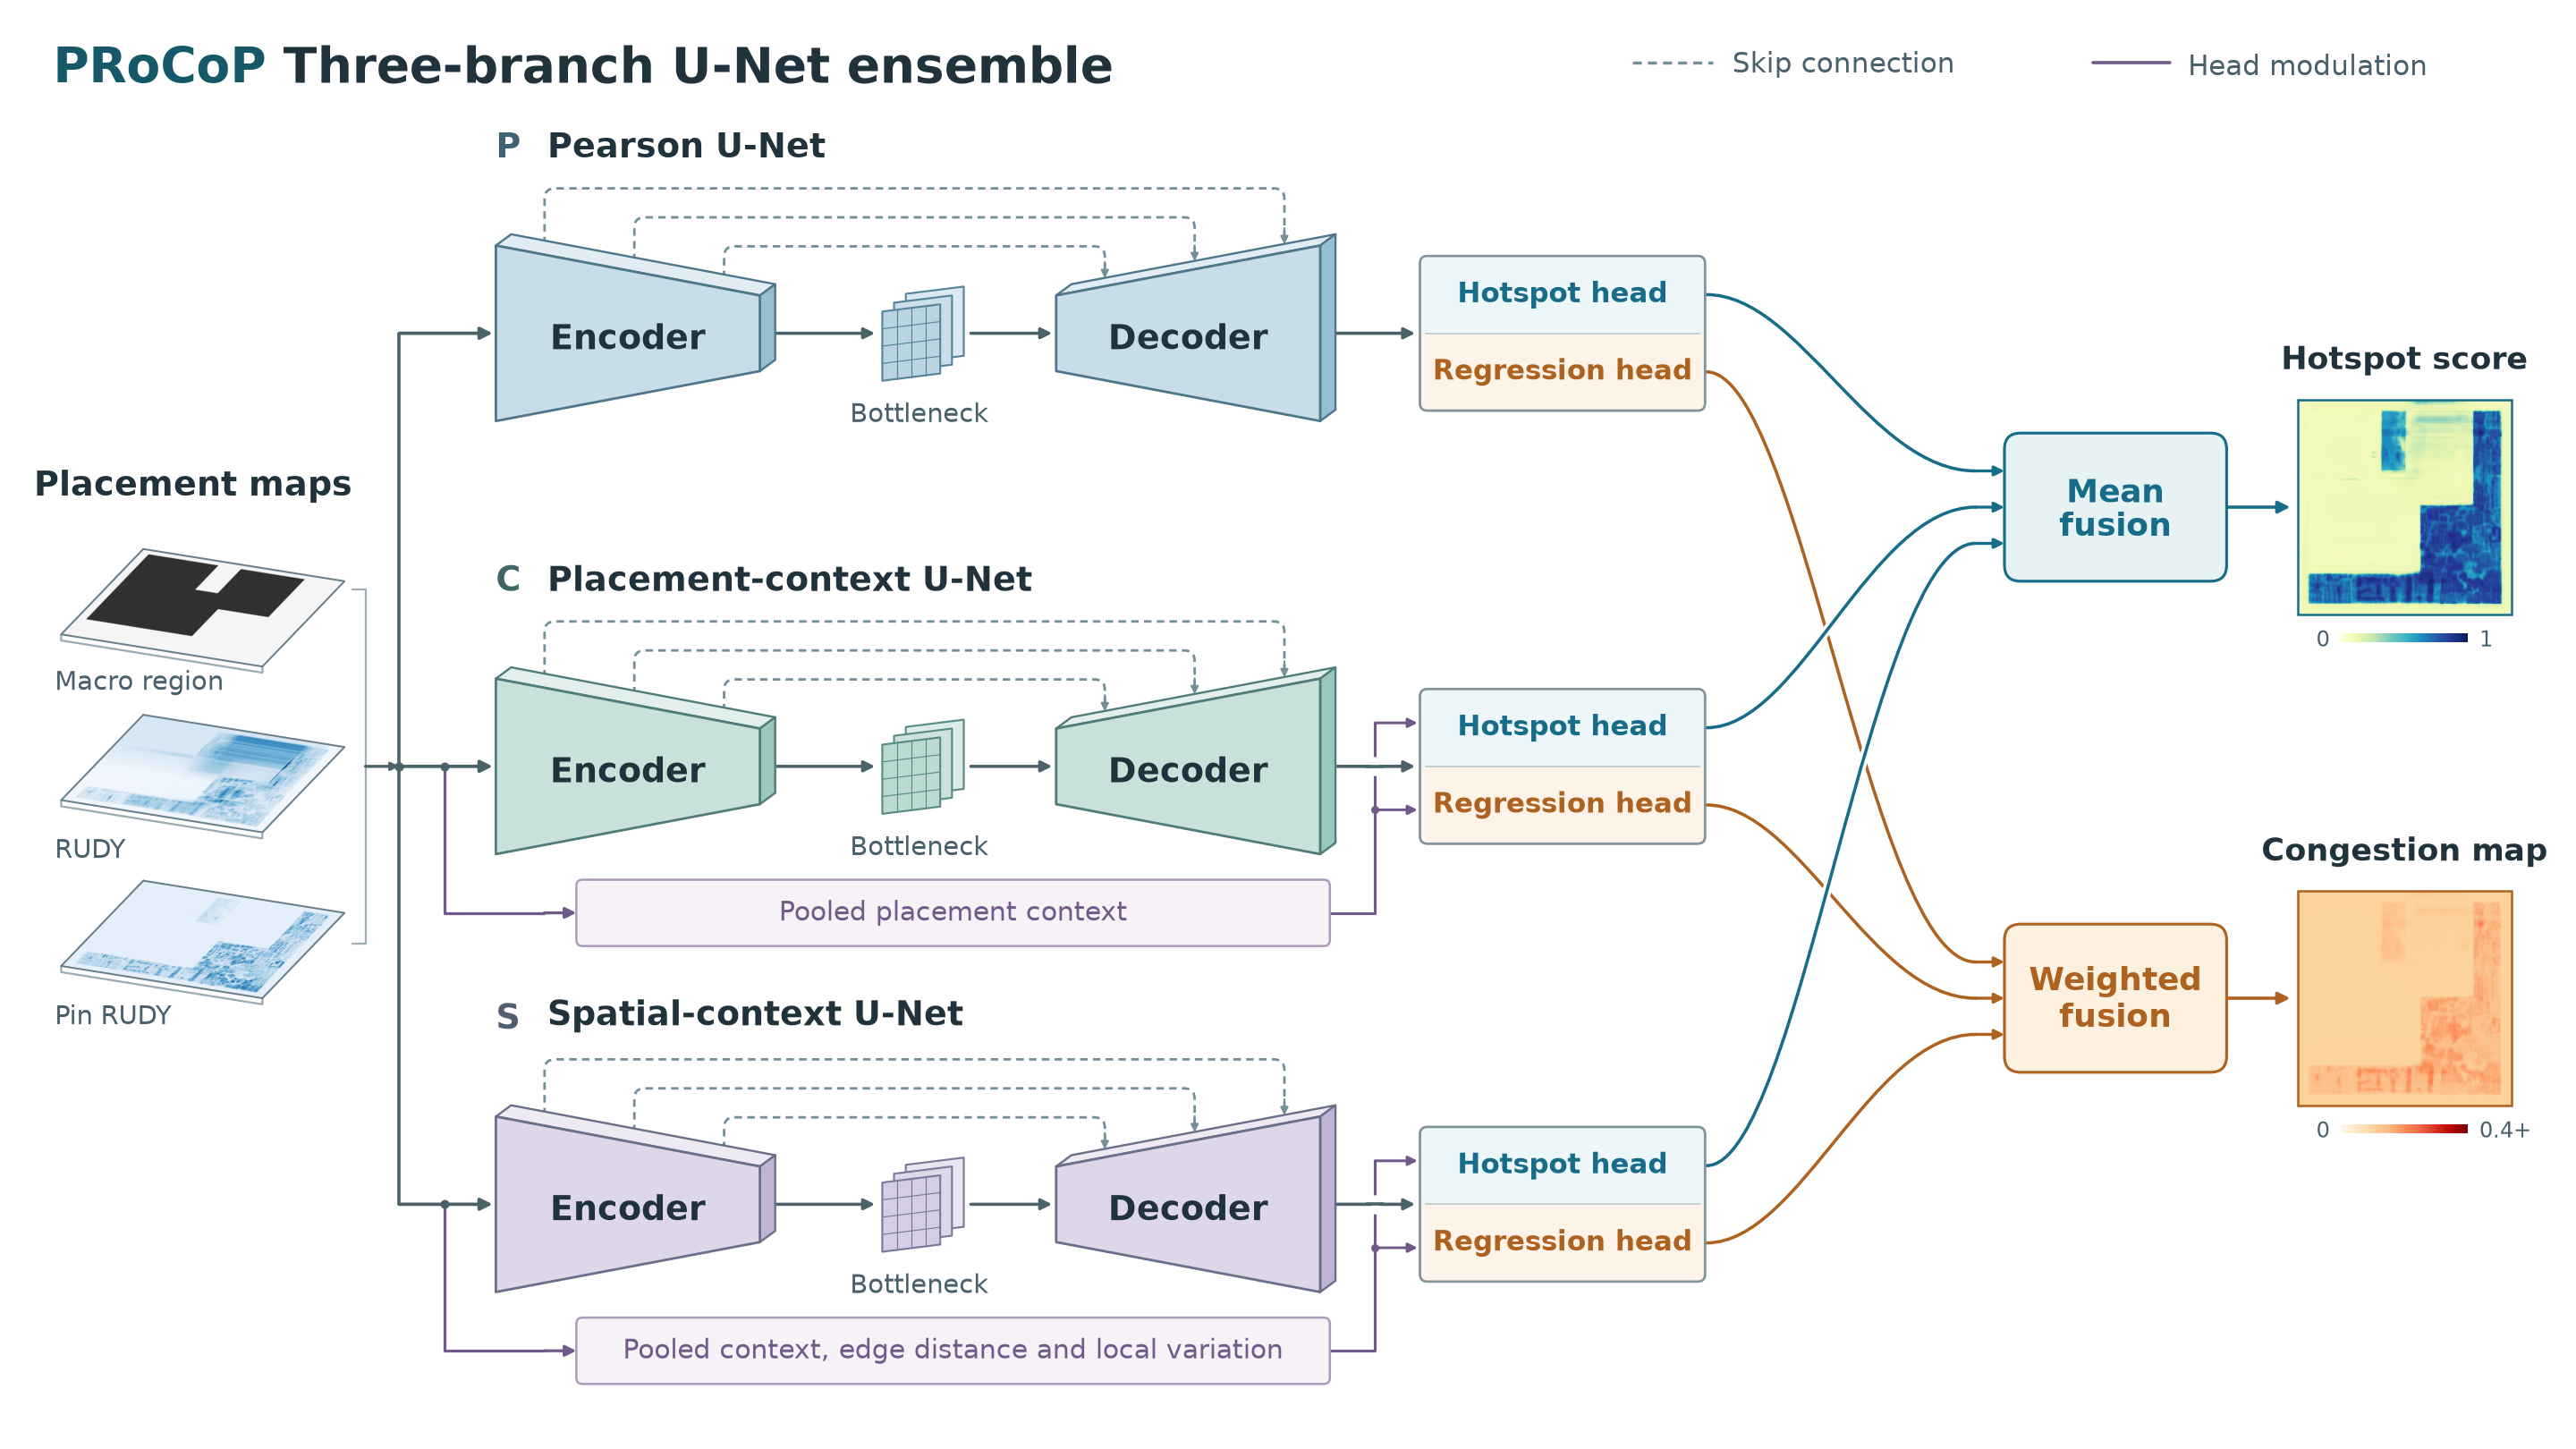
\includegraphics[width=\textwidth]{spatial_consensus_architecture.png}
\caption{Placement-to-congestion inference. All three U-Nets receive the same placement maps and have independent weights. Dashed paths carry encoder features to the matching decoder resolutions. The context pathways in C and S modulate both output heads. The ensemble averages hotspot scores across branches and gives the Pearson branch half the weight in the overflow map.}
\label{fig:architecture}
\end{figure*}

\subsection{Placement maps and supervision}
For each CircuitNet-N28 layout we read a macro-region map, RUDY, and pin RUDY~\cite{chai2022circuitnet,chai2023circuitnet}. The first locates macros, the second estimates demand across net bounding boxes, and the third describes demand at pin locations. We resize all channels and the two directional overflow maps to $256\times256$ by cubic interpolation. We min--max normalize each input channel independently within its layout. For the target $y$, we sum the resized horizontal and vertical overflows and min--max normalize the sum within that layout. Constant maps are set to zero. A high target value therefore identifies severe overflow relative to other tiles in the same layout. Recovering an absolute count of excess routing tracks would require the original scale.

Let $t$ be the 90th percentile of sampled positive training-label values. Each training layout contributes up to 2,048 values, sampled without replacement. Tile $i$ is a true hotspot if $h_i=\mathbf{1}[y_i\geq t]$. We compute $t$ once per fold and use it on every validation and test layout. Thus 10\% is a tail probability for the sampled positive training values, and the test hotspot fraction can differ by design. The RUDY baseline uses the normalized RUDY channel both as its congestion estimate and as its hotspot score.

\subsection{Baselines and objectives}
Our implementation of the CircuitNet FCN~\cite{liu2021global,chai2023circuitnet} has two pooling stages, a skip connection, and a sigmoid output (119,169 parameters). Our parameter-matched U-Net~\cite{ronneberger2015unet} has 118,725 parameters and three skip connections at full, half, and quarter resolution. Both regress $y$ using pixelwise MSE. In the FCN pilot we varied only the additional weight $\alpha$ assigned to true hotspots:
\begin{equation}
  L_{\mathrm{wMSE}} =
  \frac{\sum_i (1+\alpha h_i)(\hat y_i-y_i)^2}{\sum_i (1+\alpha h_i)}.
\end{equation}
Setting $\alpha=0$ recovers ordinary MSE. For these single-output networks, sorting predicted congestion produces the hotspot ranking.

In the dual-head U-Net, a shared decoder feeds a congestion head and a binary hotspot head. The latter predicts a score $s_i$ by applying a sigmoid to its logit. We train it with binary cross-entropy (BCE), weighting positives by the ratio of negative to positive training tiles. The Pearson branch ($P$) also penalizes disagreement between the spatial patterns of the predicted and true congestion maps. Its loss is
\begin{equation}
 L_P = L_{\mathrm{MSE}} + 0.01L_{\mathrm{BCE}} +
                  0.005(1-\rho),
\end{equation}
where $\rho$ is spatial Pearson correlation computed within a layout and averaged over eligible layouts in a minibatch. The plain dual-head ablation omits the correlation term.

\subsection{Placement context and fusion}
The context branch ($C$) uses the same loss as $P$. Congestion along a narrow row of tiles can depend on demand beyond a convolutional neighborhood. For each input channel, this branch computes $8\times8$ block means, regional means on a $4\times4$ grid, row and column means, and the layout-wide mean and standard deviation. A small convolutional module learns a spatial scale and offset for each output head from these 18 channels. The spatial branch ($S$) adds five channels: distance to the nearest horizontal and vertical die boundaries and one local standard deviation per input channel. Its loss adds $0.005(1-\widetilde{\mathrm{AP}})$, a differentiable approximation to pooled minibatch AP computed using 32 triangular score bins and up to 16,384 sampled tiles. Evaluation uses exact AP.

Each network sees the same three input maps at inference. For the three-model ensemble we combine their hotspot probabilities and congestion maps separately:
\begin{align}
 s &= (s_P+s_C+s_S)/3, \\
 \hat y &= (2\hat y_P+\hat y_C+\hat y_S)/4.
\end{align}
These weights result from averaging two existing predictors, $P+C$ and $P+S$. Each pair gives its context branch twice the weight of $P$ for hotspot scoring and averages the two maps equally. Reusing $P$ gives three forward passes and 365,318 total parameters for the ensemble.

\section{Experiments and Evaluation}
\subsection{Design splits and model selection}
The full manifest contains 10,242 layouts. In each fold we reserve all layouts of one design for testing and a second complete design for validation. The remaining four designs supply training data. Table~\ref{tab:design} identifies both reserved designs for each fold. We train the main comparisons with Adam for 15 epochs, learning rate 0.002, batch size four, seed 42, on CUDA. We keep the checkpoint with the highest validation-fold AP. For thresholded detection, we independently select the model score cutoff that maximizes validation F1, then freeze it on the test design. This score cutoff can vary across methods. The training-derived label cutoff $t$ is common to all methods within a fold.

We compared 21 methods, including single networks, feature and loss ablations, and ensembles. To assess spatial context, we first screened candidate changes on two validation designs with RISCY-FPU-b reserved as an outer test circuit. The $P+S$ pair was selected there. After observing different outcomes for $P+S$ on the first two test folds (RISCY-FPU-b and zero-riscy-b), we registered the fixed three-model average as a secondary comparison before its four remaining test outcomes were available. We report those four folds separately and repeat the outer fold with training seed 43 and the original label threshold. The code, fold definitions, and full comparison are available in the project repository.\footnote{\url{https://github.com/RickGao/PRoCoP}}

\subsection{Evaluation measures}
Our primary metric pools all tiles of one test design. Sorting scores in descending order gives precision $p_k$ and recall $r_k$ at each distinct score, with ties entering together. Average precision is $\mathrm{AP}=\sum_k (r_k-r_{k-1})p_k$. We also calculate AP within each layout that contains a hotspot. MAE averages $|\hat y_i-y_i|$ over the tiles; spatial Pearson measures agreement in the shape of each congestion map. For alarms, precision is the fraction of flagged tiles that are true hotspots, recall is the fraction of true hotspots flagged, and F1 is their harmonic mean within the fold. We average each metric equally over the six designs. This gives a small design the same influence as a design with twice as many layouts.

\begin{table*}[t]
\centering
\caption{Selected methods from the 21-method comparison. Each column is the unweighted mean of six test-design metrics (seed 42). Precision, recall, and F1 use the transferred validation cutoff. F1 is averaged after it is computed within each fold.}
\label{tab:main}
\begin{tabular}{lrrrrrrr}
\toprule
Method & Fold AP $\uparrow$ & Layout AP $\uparrow$ & MAE $\downarrow$ & Pearson $\uparrow$ & Precision (\%) & Recall (\%) & F1 (\%) \\
\midrule
RUDY & 0.19842 & 0.22701 & 0.11570 & 0.36014 & 20.14 & 55.34 & 28.83 \\
FCN, MSE & 0.25827 & 0.27824 & 0.03448 & 0.41484 & 23.46 & 53.04 & 31.42 \\
Single-head U-Net, MSE & 0.26122 & 0.28738 & 0.03425 & 0.45764 & 25.80 & 56.89 & 30.52 \\
Dual-head U-Net & 0.25985 & 0.29085 & 0.03449 & 0.43348 & 24.95 & 56.88 & 30.96 \\
Pearson branch ($P$) & 0.26944 & 0.30673 & 0.03434 & 0.48357 & 24.62 & 57.89 & 31.76 \\
Context branch ($C$) & 0.27982 & 0.31848 & 0.03437 & 0.48554 & 25.05 & 59.01 & 32.27 \\
Spatial branch ($S$) & 0.27849 & 0.31147 & 0.03515 & 0.48496 & 24.06 & 60.30 & 32.03 \\
$P+C$ & 0.28092 & 0.32090 & 0.03400 & 0.49680 & 25.23 & 58.64 & 31.89 \\
$P+S$ & 0.28106 & 0.31653 & 0.03432 & 0.49808 & 24.64 & 59.32 & 31.92 \\
$P+C+S$ & \textbf{0.28353} & \textbf{0.32243} & 0.03407 & 0.50141 & 25.24 & 58.75 & 31.94 \\
\bottomrule
\end{tabular}
\end{table*}

\subsection{Hotspot ranking and map accuracy}
The three-model ensemble achieves the highest six-fold AP among the 21 tested methods (Table~\ref{tab:main}). It gains 0.08512 absolute AP over RUDY (42.90\% relative) and 0.02526 over the FCN (9.78\% relative). It exceeds both baselines in every design, including the sparse RISCY-FPU-b fold. Its mean within-layout AP is 0.32243. This matters when an engineer inspects one placement at a time. The six-fold MAE improvement over the FCN is smaller, from 0.03448 to 0.03407. Two earlier ensembles that calibrated regression weights on validation attained the lowest mean MAE (0.03395).

\begin{table*}[t]
\centering
\caption{Leave-one-design-out results. Hotspots is the fraction of test tiles meeting the training-derived label cutoff. AP columns use identical layouts and labels within each row.}
\label{tab:design}
\begin{tabular}{llrrrrrr}
\toprule
Test design & Validation design & Test layouts & Hotspots (\%) & RUDY AP & FCN AP & $P+C$ AP & $P+C+S$ AP \\
\midrule
zero-riscy-b & RISCY-FPU-b & 1,122 & 5.97 & 0.08046 & 0.06901 & 0.12118 & 0.12094 \\
RISCY-a & RISCY-FPU-a & 2,003 & 12.80 & 0.32045 & 0.43470 & 0.44955 & 0.45168 \\
zero-riscy-a & RISCY-b & 2,042 & 11.58 & 0.29592 & 0.40910 & 0.43421 & 0.43238 \\
RISCY-b & zero-riscy-b & 1,858 & 5.98 & 0.08575 & 0.11116 & 0.12880 & 0.13555 \\
RISCY-FPU-b & RISCY-b & 1,248 & 3.27 & 0.05426 & 0.07978 & 0.09544 & 0.09997 \\
RISCY-FPU-a & RISCY-b & 1,969 & 13.84 & 0.35365 & 0.44588 & 0.45636 & 0.46069 \\
\bottomrule
\end{tabular}
\end{table*}

\subsection{What accounts for the gain?}
Replacing the FCN with a similarly sized U-Net increases mean AP from 0.25827 to 0.26122. Adding an unconditioned hotspot head alone yields 0.25985. With the same dual-head architecture, adding the correlation term raises AP to 0.26944. Adding pooled context raises it further to 0.27982, the highest AP of a single network in this study. Adding the edge and local-variation features together with the soft-AP loss gives 0.27849 for $S$ alone. That comparison changes two factors at once. In the two-design validation screen, the $P+C$ pair scored 0.27307, spatial features alone scored 0.27457, and spatial features with soft AP scored 0.27887.

The gain from adding a third network is smaller. Mean AP rises from 0.28092 for $P+C$ to 0.28353 for $P+C+S$, at the cost of one extra forward pass. On the four folds evaluated after registering the ensemble, these averages were 0.36723 and 0.37007. On RISCY-FPU-b with seed 43, $P+C$ reached 0.09644 and the ensemble 0.09593, reversing their seed-42 ordering. The two-pass model therefore remains a reasonable choice when inference cost matters.

\subsection{Ranking versus alarms}
At validation-selected cutoffs the three-model ensemble averages 25.24\% precision and 58.75\% recall, compared with 23.46\% and 53.04\% for the FCN. Its mean F1 is 31.94\%. A hard-negative ranking variant achieved the best F1 of the 21 methods (32.75\%) with AP of only 0.25564. The two metrics answer different design questions: which tiles to inspect first, and what fraction of alarms can be trusted after a cutoff transfers to another circuit.

\begin{figure*}[!t]
\centering
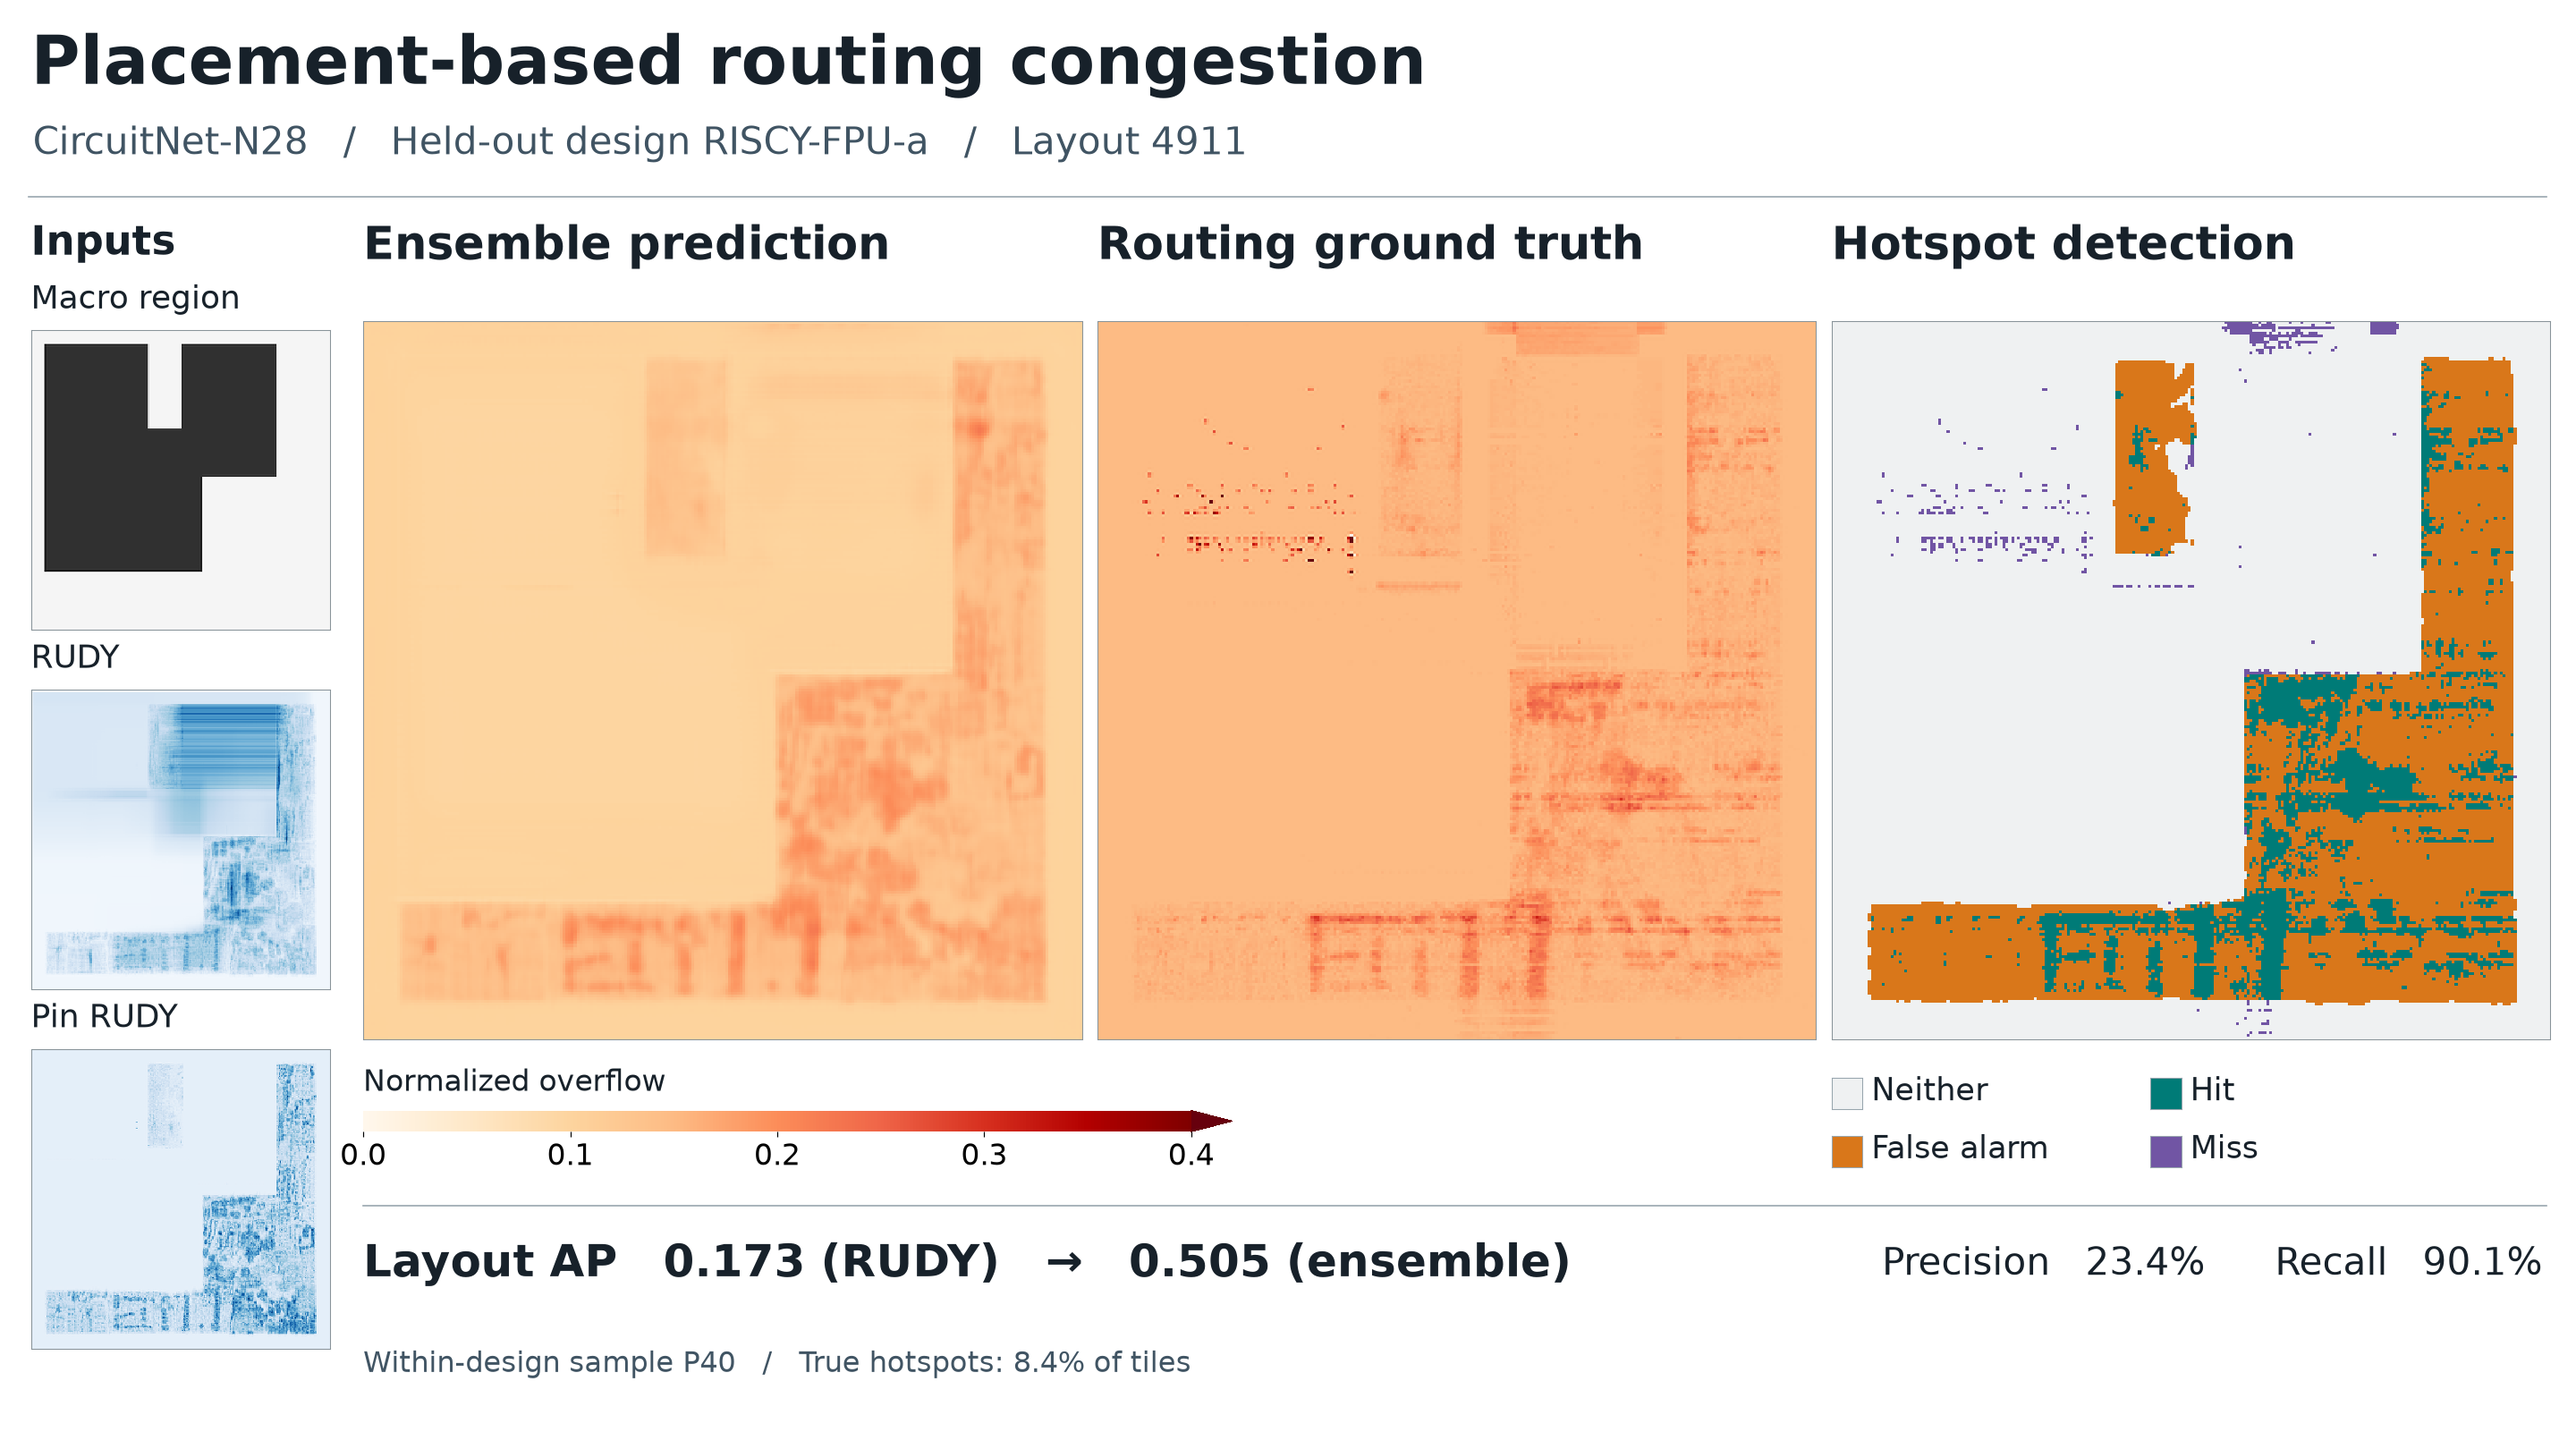
\includegraphics[width=.88\textwidth]{02_4911-RISCY-FPU-a-2-c5-u0.png}\par\smallskip
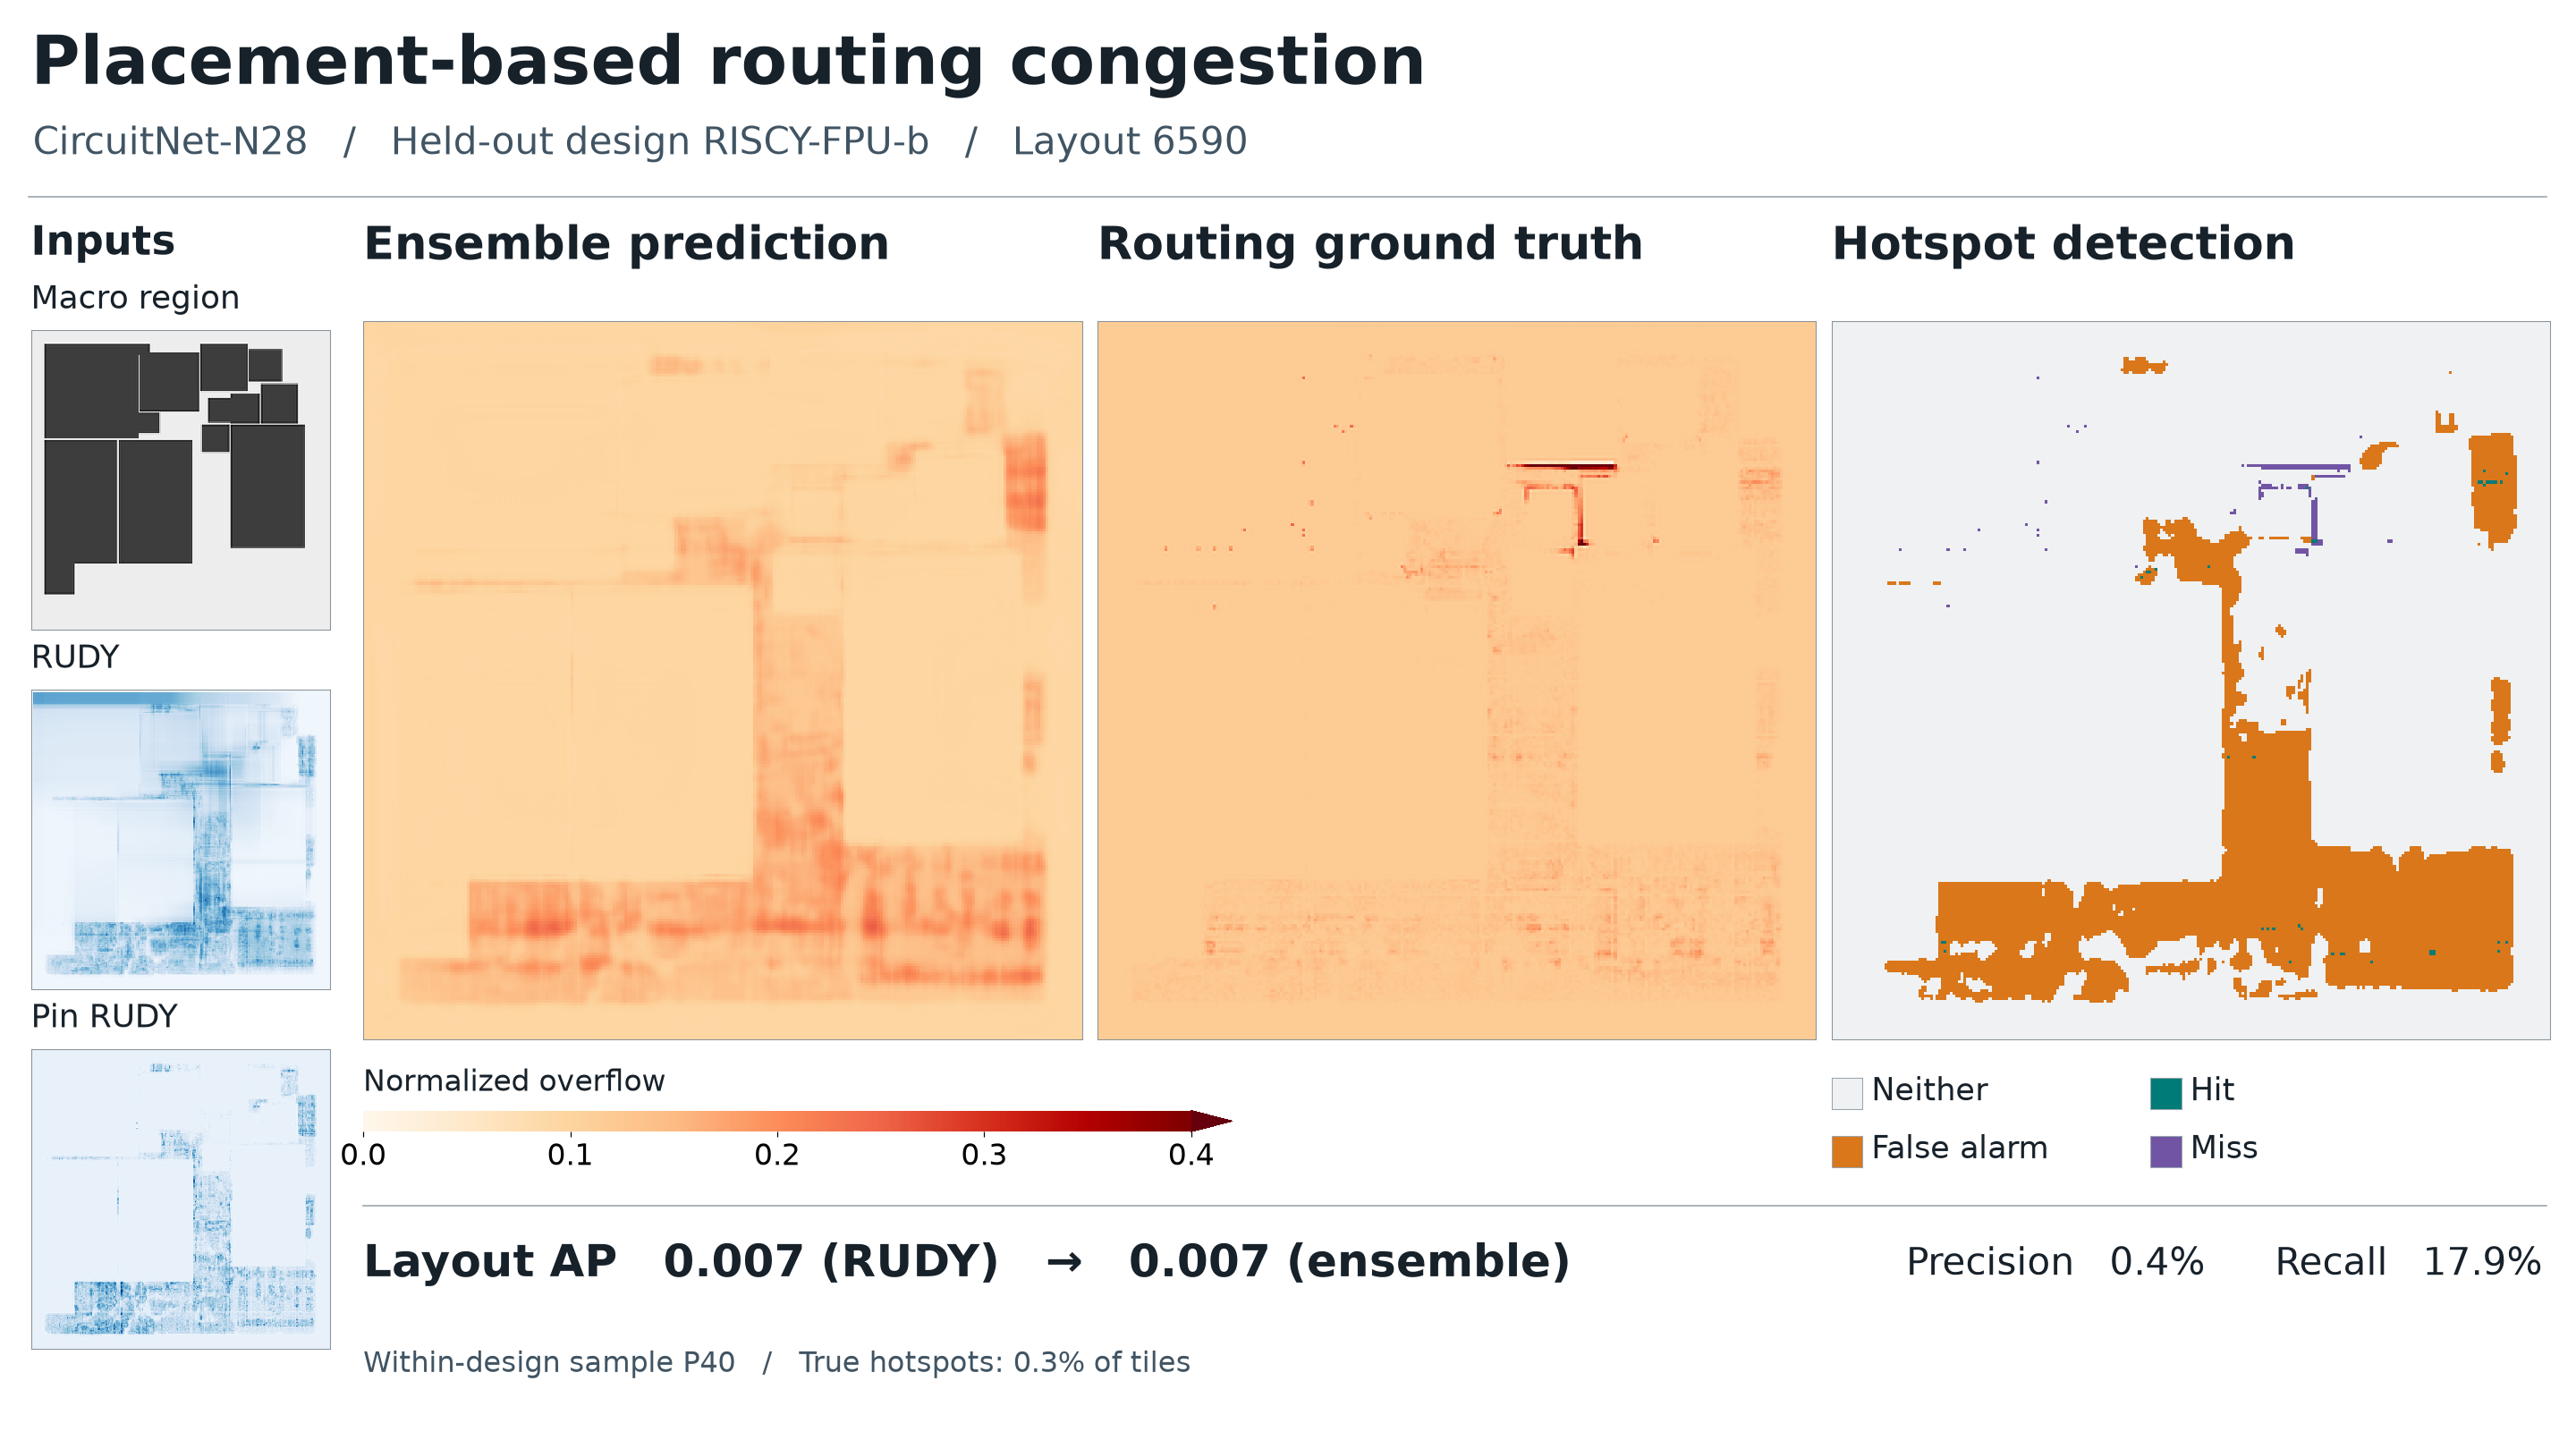
\includegraphics[width=.88\textwidth]{02_6590-RISCY-FPU-b-2-c5-u0.png}
\caption{Held-out predictions for RISCY-FPU-a layout 4911 (top) and RISCY-FPU-b layout 6590 (bottom). Each example occupies the 40th-percentile rank by layout AP within its design's gallery candidate set. Prediction and routed overflow share a color scale. In the detection overlay, teal marks hits, orange marks false alarms, and purple marks missed hotspots.}
\label{fig:layout}
\end{figure*}

Figure~\ref{fig:layout} shows how differently the validation cutoffs transfer. On layout 4911, ensemble AP is 0.505, up from 0.173 for RUDY. At the transferred cutoff it finds 4,951 of 5,495 true hotspot tiles (90.1\% recall), but flags 21,176 tiles in all (23.4\% precision). On layout 6590, only 224 of 65,536 tiles are true hotspots. The model finds 40 of them among 11,391 flags (17.9\% recall, 0.35\% precision). Its AP of 0.0072 is close to RUDY's 0.0068. The second example illustrates how a sparse layout can yield many false alarms even when its fold has a positive average AP gain over RUDY.

\subsection{Revisiting weighted regression}
In the early zero-riscy-b FCN pilot (128 training, 32 validation, and 32 test layouts), both checkpoints were selected by validation MAE. Changing $\alpha$ from 0 to 3 shifted test MAE from 0.03082 to 0.03011 and F1 from 0.77\% to 4.62\% at the pilot's fixed cutoff. In a later full-data single-head U-Net validation sweep, the best AP for $\alpha=0,1,3$ was 0.08596, 0.07952, and 0.08239, respectively. Regression weighting thus helped one small-sample operating point. The full-data validation ranking favored ordinary MSE for the single-head baseline. These observations motivated learning a separate hotspot score.

\subsection{Comparison with published results and limitations}
The CLDRoute release~\cite{thorat2026cldroute} permits a narrower comparison on the same 1,122 zero-riscy-b test layouts. The three-channel pixel-diffusion baseline reports full-map Pearson of 0.3077 and MAE of 0.02730. Our three-channel ensemble reaches 0.35162 and 0.02758. The ten-channel conditional latent diffusion model reaches Pearson of 0.3687, an absolute advantage of 0.01708 over ours. The authors average three seeds and use additional conditioning in the ten-channel case. Their congestion results do not report AP with our hotspot definition, so these values support a comparison of map quality only.

Test hotspot prevalence ranges from 3.27\% to 13.84\% (Table~\ref{tab:design}). Because the AP of an uninformative constant score equals prevalence, part of the raw difference between designs reflects how rare their hotspots are. Repeated layouts of the same circuit provide many test tiles but only six held-out design identities. The designs also share RISC-V families, and the second training seed covers only one circuit. Finally, per-layout normalization removes absolute overflow severity, and our offline evaluation measures neither routed wirelength nor the effect of changing a placement in response to an alarm.

\clearpage
\section{Conclusion}
A placement-context U-Net ranks congestion hotspots more accurately than the FCN on average, and a fixed three-model ensemble improves on both the FCN and RUDY in every held-out design. Most of the improvement is available from one context-aware network. The third network gives the best six-design mean AP, with a smaller and seed-sensitive gain over a two-network predictor. For use inside a placer, the remaining question is whether a designer can transfer an alarm threshold with acceptable false-alarm cost, particularly on circuits whose hotspots are sparse.

\bibliographystyle{IEEEtran}
\bibliography{refs}
\end{document}
